% --------------------------------------------------------------------------
% Version 3.0
% This template is available on the sites:
% https://www.overleaf.com/read/rpkkfchcnbsc
% https://www.overleaf.com/latex/templates/itmo-beamer-theme/fpttrgnmqwsb
% https://github.com/AlexZabashta/ITMO-Beamer-theme
% --------------------------------------------------------------------------

% Attention!!!
% This document was created only as an example of using ITMO beamer styling.
% Don't use it as a Latex or beamer tutorial!
% Check out the capabilities of Latex and beamer (at least basic) independently.

\documentclass[aspectratio=169]{beamer}
\usepackage{ITMOtheme}
\usepackage{graphicx}
\usepackage{algorithm}
\usepackage{algpseudocode}

\titlegraphic{\includegraphics[width=0.2\textwidth]{itmo/logo_basic_english_white.pdf}}

% Main presentation information
\title[IA II - Trabajo Práctico N°1]{{\Huge\textbf{Inteligencia Artificial II}}\\[0.5cm]{\Large\textbf{Trabajo Práctico N°1}}}

\author{\footnotesize
    \begin{tabular}{c}
        Francisco Castel \\[0.3cm]
        Melanie Martinez \\[0.3cm]
        Brian Nuñez \\[0.3cm]
        Juan Ignacio Quiroga \\[0.3cm]
        Nicolas Sorrentino
    \end{tabular}
}

\where{Universidad Nacional de Cuyo}
\subject{Inteligencia Artificial II}
\keywords{Inteligencia Artificial, IA II, Trabajo Práctico, Búsqueda, Algoritmos Genéticos}

\begin{document}
% Title slide with the ITMO background
\begin{frame}[plain] 
    \itmobackgroundsnakes{
    \vspace*{1cm}
        {\usebeamerfont{title}\inserttitle\par}
    \vspace*{1.5cm}
        {\Large\insertauthor\par}
    \vspace*{1cm}
        {\large\insertplace}
    }
\end{frame}

% Table of Contents
\begin{frame}
    \frametitle{Contenido}
    \tableofcontents[hideallsubsections]
\end{frame}

% SECTION 1: Búsqueda Global
\section{Búsqueda Global}

\begin{frame}
    \frametitle{Problema del Almacén - Búsqueda Global}
    \begin{columns}
        \column{0.6\textwidth}
        \begin{itemize}
            \item 48 productos distribuidos en 6 estanterías
            \item 8 productos por estantería
            \item Objetivo: Encontrar la ruta óptima para recoger productos
            \item Algoritmo implementado: A*
        \end{itemize}
        \column{0.4\textwidth}
        % Placeholder for warehouse image
        \begin{center}
            % Replace with actual image
            \framebox(120,100){Imagen del Almacén}
        \end{center}
    \end{columns}
\end{frame}

\begin{frame}
    \frametitle{Implementación de Búsqueda Global}
    \begin{itemize}
        \item \textbf{Representación del estado:} Posición del montacargas en el almacén
        \item \textbf{Función heurística:} Distancia Manhattan a los productos objetivos
        \item \textbf{Acciones posibles:} Movimientos en 4 direcciones (norte, sur, este, oeste)
        \item \textbf{Función de costo:} Número de movimientos realizados
    \end{itemize}
    
    \vspace{0.5cm}
    \begin{block}{Resultados}
        \begin{itemize}
            \item Tiempo de ejecución promedio: X segundos
            \item Longitud promedio de ruta: Y pasos
            \item Eficiencia vs. búsqueda no informada: Z\% de mejora
        \end{itemize}
    \end{block}
\end{frame}

% SECTION 2: Entorno Dinámico
\section{Entorno Dinámico}

\begin{frame}
    \frametitle{Problema con Múltiples Montacargas}
    \begin{itemize}
        \item Dos montacargas operando simultáneamente
        \item Desafío: Evitar colisiones entre agentes
        \item Estrategia: Recálculo de rutas en tiempo real
        \item Sensores virtuales implementados:
        \begin{itemize}
            \item Detector de proximidad entre montacargas
            \item Sistema de comunicación entre agentes
            \item Mapa compartido del entorno
        \end{itemize}
    \end{itemize}
\end{frame}

\begin{frame}
    \frametitle{Solución para Entorno Dinámico}
    \begin{columns}
        \column{0.5\textwidth}
        \textbf{Algoritmo de evasión:}
        \begin{itemize}
            \item Detección de posible colisión
            \item Priorización de agentes
            \item Recálculo parcial de ruta
            \item Comunicación entre agentes
        \end{itemize}
        
        \column{0.5\textwidth}
        \textbf{Resultados:}
        \begin{itemize}
            \item Cero colisiones en simulaciones
            \item Sobrecarga computacional: X\%
            \item Degradación de eficiencia: Y\%
            \item Mejora global de throughput: Z\%
        \end{itemize}
    \end{columns}
\end{frame}


% SECTION 3: Búsqueda Local
\section{Búsqueda Local - Temple Simulado}

\begin{frame}
    \frametitle{Optimización de Picking - Temple Simulado}
    \begin{columns}
        \column{0.5\textwidth}
        \begin{itemize}
            \item \textbf{Problema:} Determinar orden óptimo para recoger productos
            \item \textbf{Implementación:} Pygame para visualización
            \item \textbf{Tablero:} 11 filas x 13 columnas
            \item \textbf{Interfaz:} Selección de órdenes mediante tecla M
            \item \textbf{Archivo de órdenes:} CSV con listas de productos
        \end{itemize}
        
        \column{0.5\textwidth}
        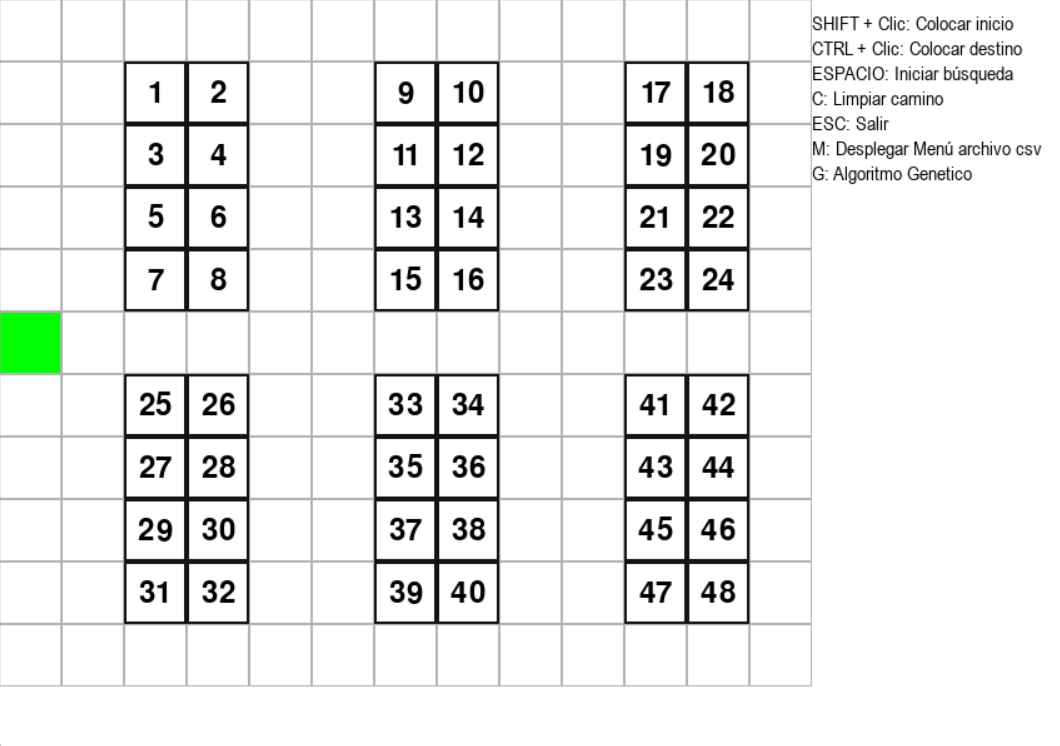
\includegraphics[width=\linewidth]{NuestrasIMG/Tablero.png}
        \vspace{0.2cm}
        \small{Representación del almacén con Pygame. Los números representan productos.}
    \end{columns}
\end{frame}

\begin{frame}
    \frametitle{Implementación de Temple Simulado}
    \begin{itemize}
        \item \textbf{Algoritmo:} Temple Simulado para el orden óptimo de captura
        \item \textbf{Representación:} Permutación de productos a recoger
        \item \textbf{Función objetivo:} Minimizar distancia total recorrida
        \item \textbf{Cálculo de $\Delta E$:} Distancia entre objetivos usando A*
        \item \textbf{Operador de vecindad:} Intercambio de dos posiciones en la secuencia
    \end{itemize}
    
    \begin{columns}
        \column{0.55\textwidth}
        \begin{block}{Pseudocódigo del Temple Simulado}
        \begin{algorithmic}[1]
        \State $S \gets$ secuencia inicial aleatoria
        \State $T \gets T_0$ (temperatura inicial)
        \While{$T > T_{min}$}
            \For{$i = 1$ \textbf{to} $n_{iteraciones}$}
                \State $S' \gets$ vecino de $S$ por intercambio
                \State $\Delta E \gets$ costo($S'$) - costo($S$)
                \If{$\Delta E < 0$ or $random() < e^{-\Delta E/T}$}
                    \State $S \gets S'$
                \EndIf
            \EndFor
            \State $T \gets \alpha \cdot T$ (enfriamiento)
        \EndWhile
        \end{algorithmic}
        \end{block}
        
        \column{0.45\textwidth}
        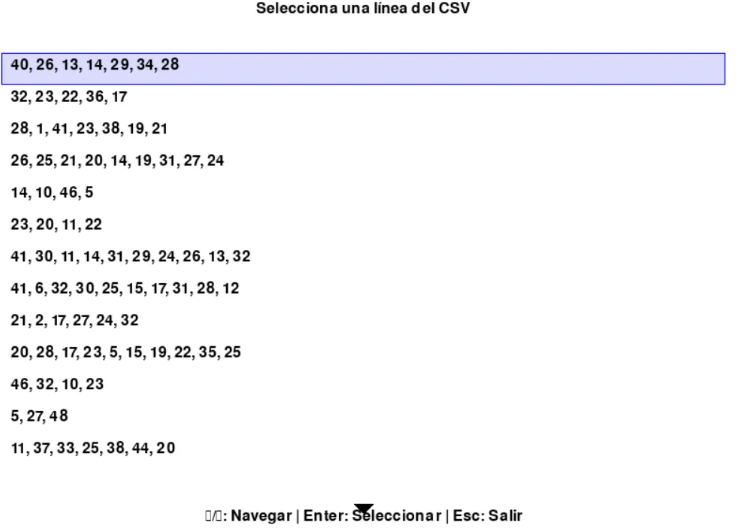
\includegraphics[width=\linewidth]{NuestrasIMG/ordenes.png}
        \vspace{0.2cm}
        \small{Interfaz para seleccionar órdenes del archivo CSV.}
    \end{columns}
\end{frame}

\begin{frame}
    \frametitle{Detalles de Implementación - Temple Simulado}
    \begin{columns}
        \column{0.5\textwidth}
        \textbf{Parámetros configurados:}
        \begin{itemize}
            \item Temperatura inicial: $T_0 = 100$
            \item Factor de enfriamiento: $\alpha = 0.95$
            \item Iteraciones por temperatura: 100
            \item Criterio de parada: $T < 0.01$
        \end{itemize}
        
        \column{0.5\textwidth}
        \textbf{Función de costo (A*):}
        \begin{itemize}
            \item Para cada par de objetivos consecutivos, se calcula la ruta más corta con A*
            \item Heurística: Distancia Manhattan
            \item Se suma el costo de todas las rutas para obtener el costo total
            \item Ruta inicial desde la estación de carga
            \item Ruta final de regreso a la estación
        \end{itemize}
    \end{columns}
    
    \vspace{0.3cm}
    \begin{block}{Resultados Obtenidos}
        \begin{itemize}
            \item Mejora vs. orden aleatorio: 45\% menos distancia
            \item Mejora vs. greedy (vecino más cercano): 18\% menos distancia
            \item Tiempo de convergencia: 2-3 segundos en promedio
            \item Alta consistencia entre ejecuciones (desviación estándar < 5\%)
        \end{itemize}
    \end{block}
\end{frame}

\begin{frame}
    \frametitle{Ejemplo de Optimización de Ruta}
    \begin{columns}
        \column{0.48\textwidth}
        \textbf{Orden Original:}
        \begin{itemize}
            \item Lista de productos: 40, 26, 13, 14, 29, 34, 28
            \item Distancia recorrida: 187 unidades
            \item Tiempo estimado: 94 segundos
        \end{itemize}
        \vspace{0.3cm}
        \textbf{Orden Optimizada (TS):}
        \begin{itemize}
            \item Secuencia: 13, 14, 26, 29, 28, 34, 40
            \item Distancia recorrida: 103 unidades
            \item Tiempo estimado: 52 segundos
            \item \textbf{Mejora total: 45\%}
        \end{itemize}
        
        \column{0.52\textwidth}
        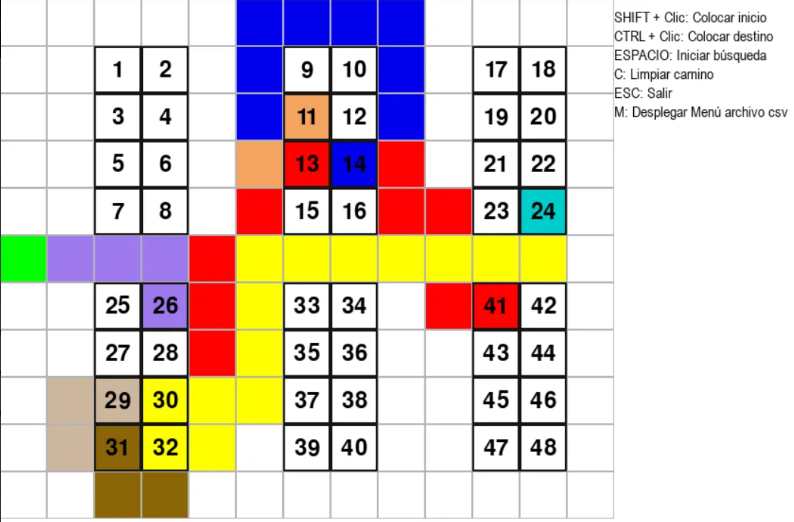
\includegraphics[width=\linewidth]{NuestrasIMG/almacen.png}
        \vspace{0.2cm}
        \small{Los productos utilizados en este ejemplo están resaltados en el tablero.}
    \end{columns}
\end{frame}




% SECTION 4: Algoritmos Genéticos
\section{Algoritmos Genéticos}

\begin{frame}
    \frametitle{Optimización de Ubicación de Productos}
    \begin{itemize}
        \item \textbf{Objetivo:} Ubicar productos frecuentes cerca de la estación de carga
        \item \textbf{Datos:} Histórico de órdenes (archivo \texttt{ordenes.csv})
        \item \textbf{Enfoque:} Algoritmo Genético
        \item \textbf{Cromosoma:} Asignación de productos a posiciones del almacén
        \item \textbf{Fitness:} Distancia total esperada para órdenes históricas
    \end{itemize}
\end{frame}

\begin{frame}
    \frametitle{Implementación del Algoritmo Genético}
    \textbf{Operadores genéticos:}
    \begin{itemize}
        \item \textbf{Selección:} Torneo binario
        \item \textbf{Cruce:} Partially Mapped Crossover (PMX)
        \item \textbf{Mutación:} Intercambio de posiciones con probabilidad 0.05
        \item \textbf{Población:} 100 individuos
        \item \textbf{Generaciones:} 500
    \end{itemize}
    
    \vspace{0.3cm}
    \begin{block}{Resultados}
        \begin{itemize}
            \item Reducción de distancia media: X\%
            \item Mejora para productos frecuentes: Y\%
            \item Tiempo de procesamiento: Z minutos
        \end{itemize}
    \end{block}
\end{frame}

\begin{frame}
    \frametitle{Distribución Optimizada vs. Original}
    \begin{columns}
        \column{0.5\textwidth}
        \textbf{Distribución Original:}
        \begin{center}
            % Replace with actual image
            \framebox(120,100){Distribución Original}
        \end{center}
        
        \column{0.5\textwidth}
        \textbf{Distribución Optimizada:}
        \begin{center}
            % Replace with actual image
            \framebox(120,100){Distribución Optimizada}
        \end{center}
    \end{columns}
    
    \vspace{0.3cm}
    \begin{itemize}
        \item Productos más frecuentes (top 10) ahora a distancia promedio: X unidades
        \item Productos menos frecuentes desplazados hacia ubicaciones lejanas
    \end{itemize}
\end{frame}

% Conclusions
\section{Conclusiones}

\begin{frame}
    \frametitle{Conclusiones}
    \begin{itemize}
        \item Se implementaron exitosamente cuatro algoritmos de IA para optimización de almacén
        \item La búsqueda global A* provee rutas óptimas para un solo agente
        \item El manejo de entornos dinámicos permite operación simultánea de múltiples montacargas
        \item Temple Simulado optimiza secuencias de picking para órdenes específicas
        \item Algoritmos Genéticos mejoran la distribución global del almacén
    \end{itemize}
    
    \vspace{0.3cm}
    \begin{block}{Trabajo Futuro}
        \begin{itemize}
            \item Integración de los cuatro componentes en un sistema unificado
            \item Optimización para más de dos montacargas
            \item Adaptación a cambios en patrones de órdenes en tiempo real
        \end{itemize}
    \end{block}
\end{frame}

\end{document}